\chapter{Interface utilisateur\\ (Adrian)}

Nous avons rapidement mis en place une interface graphique simple et
fonctionnelle, afin de tester nos parties et nos différentes implémentations
efficacement. La bibliothèque SDL est assez limitée en termes d'interface
utilisateur, c'est pourquoi nous avons utilisé la bibliothèque GTK+ pour cette
tâche.

Cependant, écrire une interface en dur dans le code est un processus fastidieux
et source d'erreurs. GTK+ contourne ce problème en permettant de charger une
description XML de l'interface. L'outil de design d'interface utilisateur
\textit{Glade} nous donne la possibilité de créer cette interface en quelques
minutes et de l'exporter en format XML lisible par GTK+.

\begin{figure}[H]
    \centering
    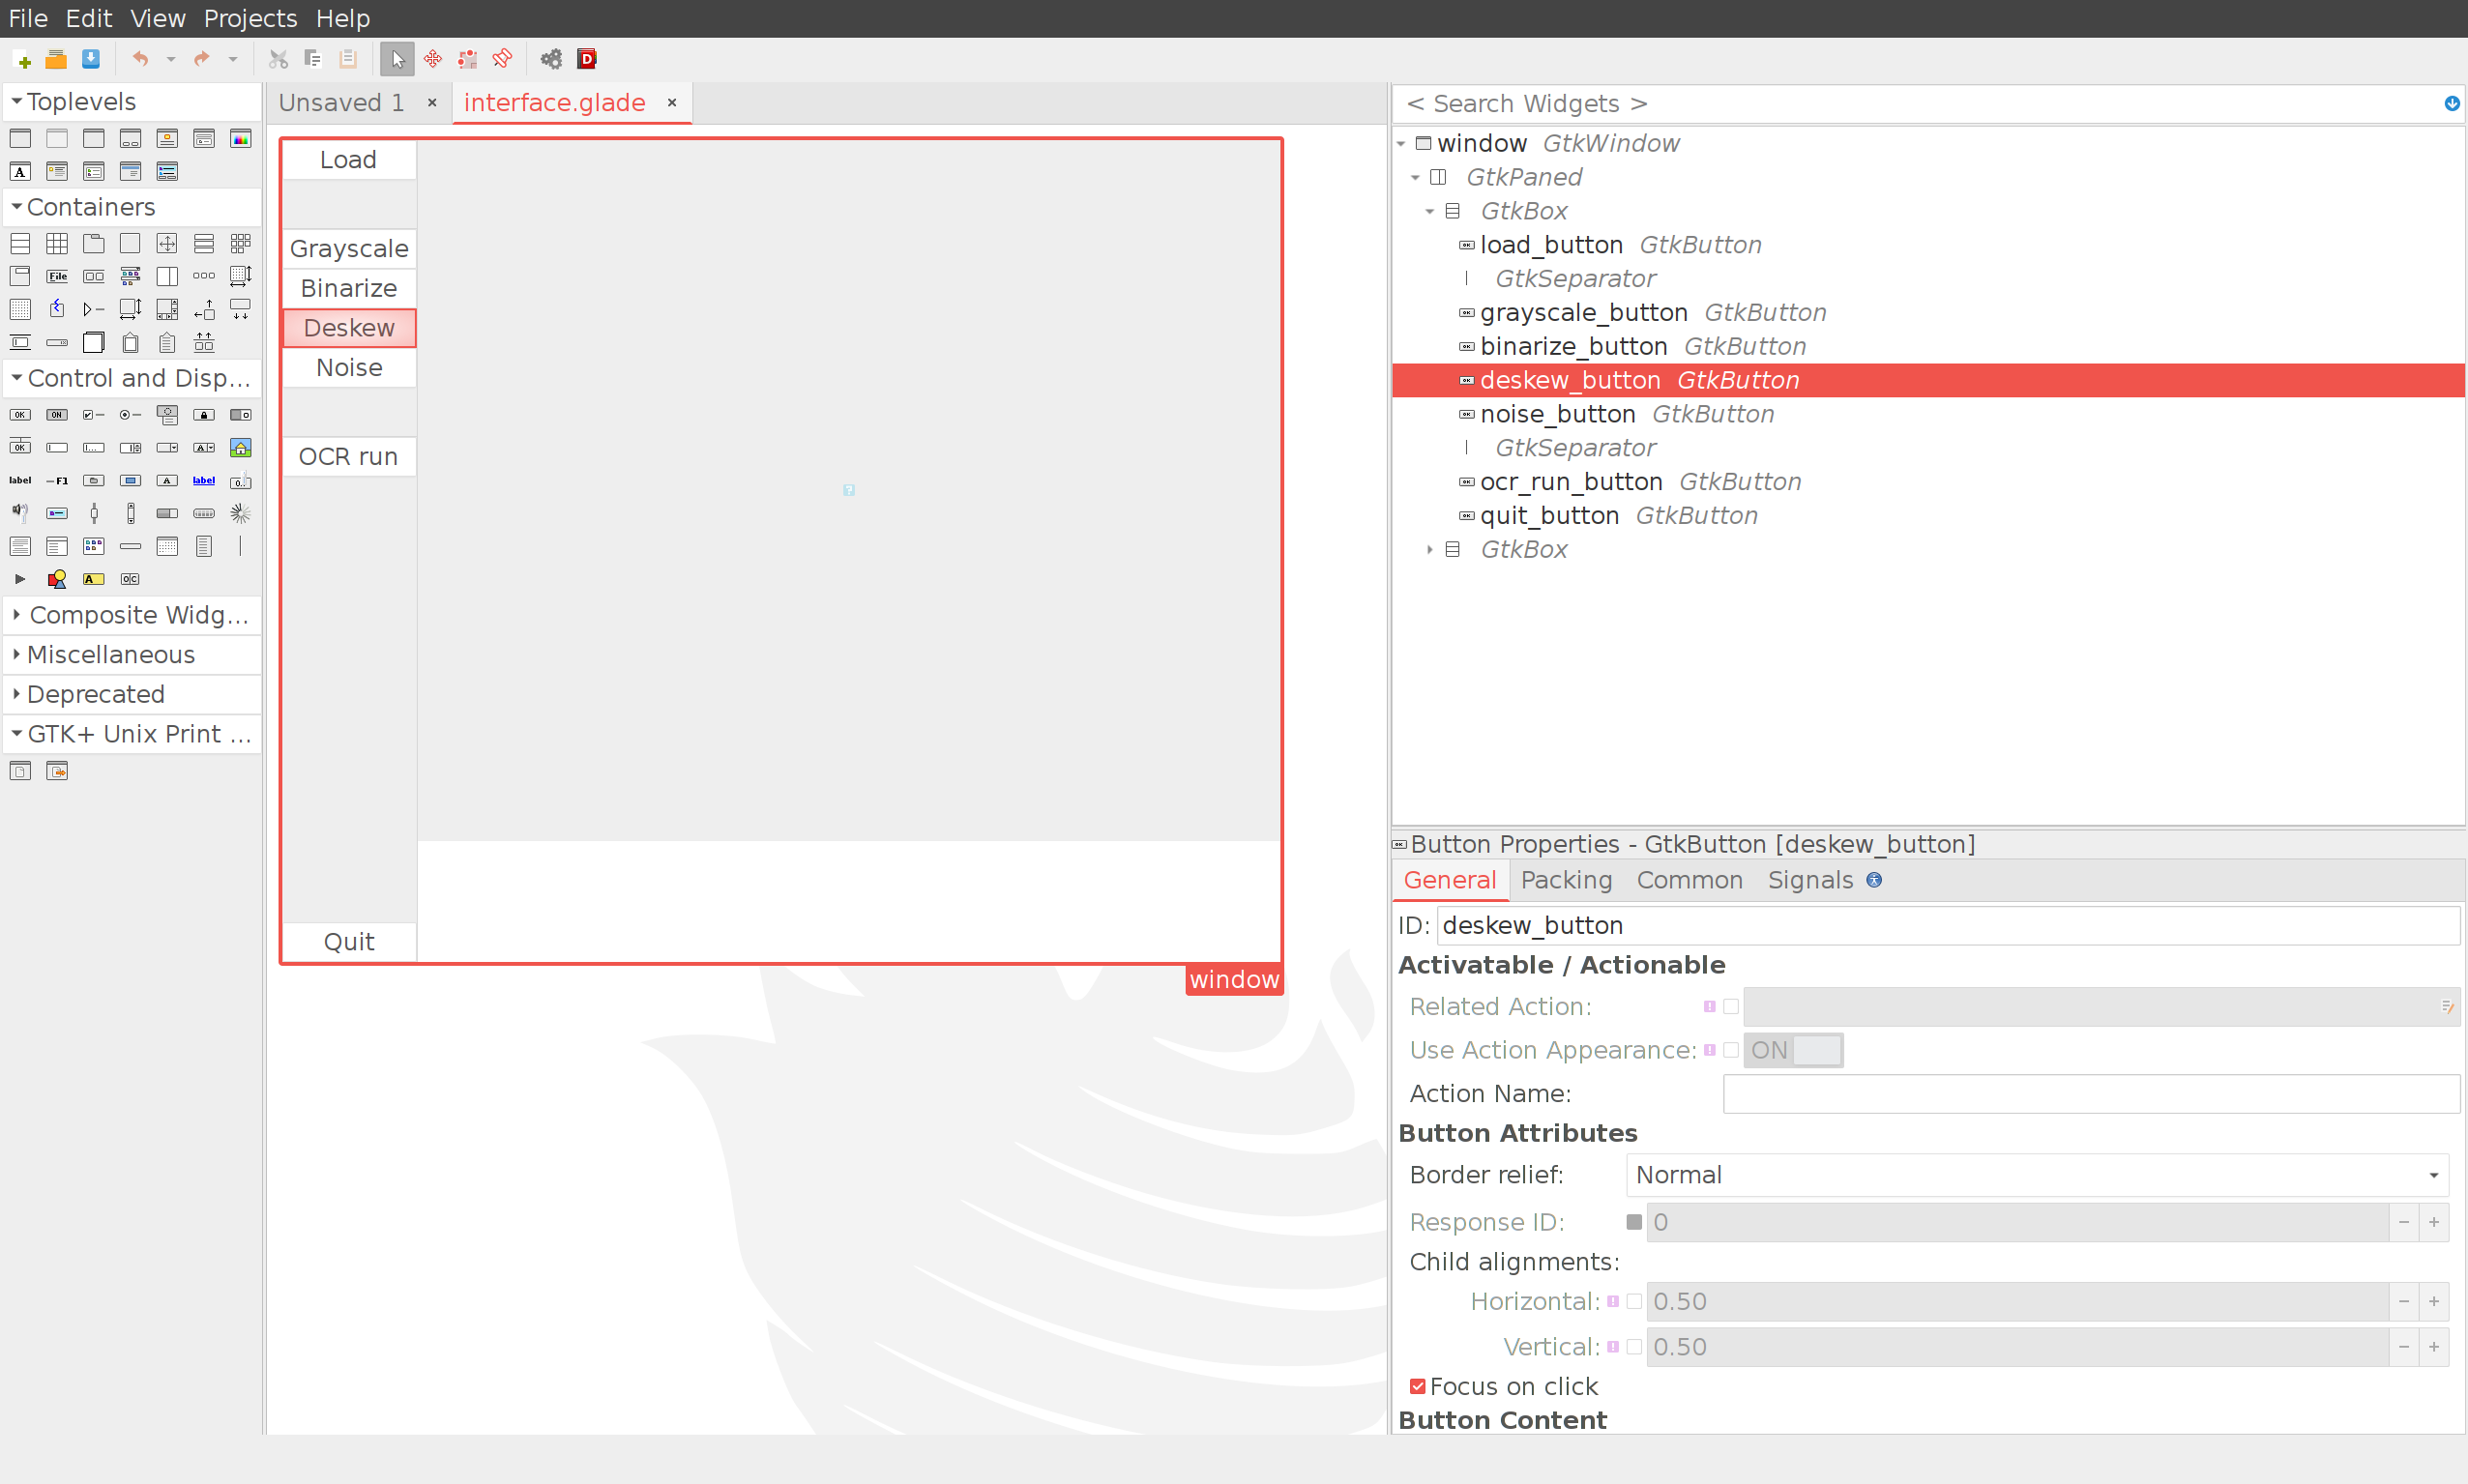
\includegraphics[width=0.7\textwidth]{glade}
    \caption{Conception de l'interface dans Glade}
\end{figure}

L'interface est alors composée des boutons d'utilisation sur le menu gauche
(pour charger l'image, la pré-traiter, et lancer l'OCR dessus), ainsi que de
l'image actuellement chargée en mémoire au centre de l'écran, et enfin la sortie
textuelle de l'OCR en bas :

\begin{figure}[H]
    \centering
    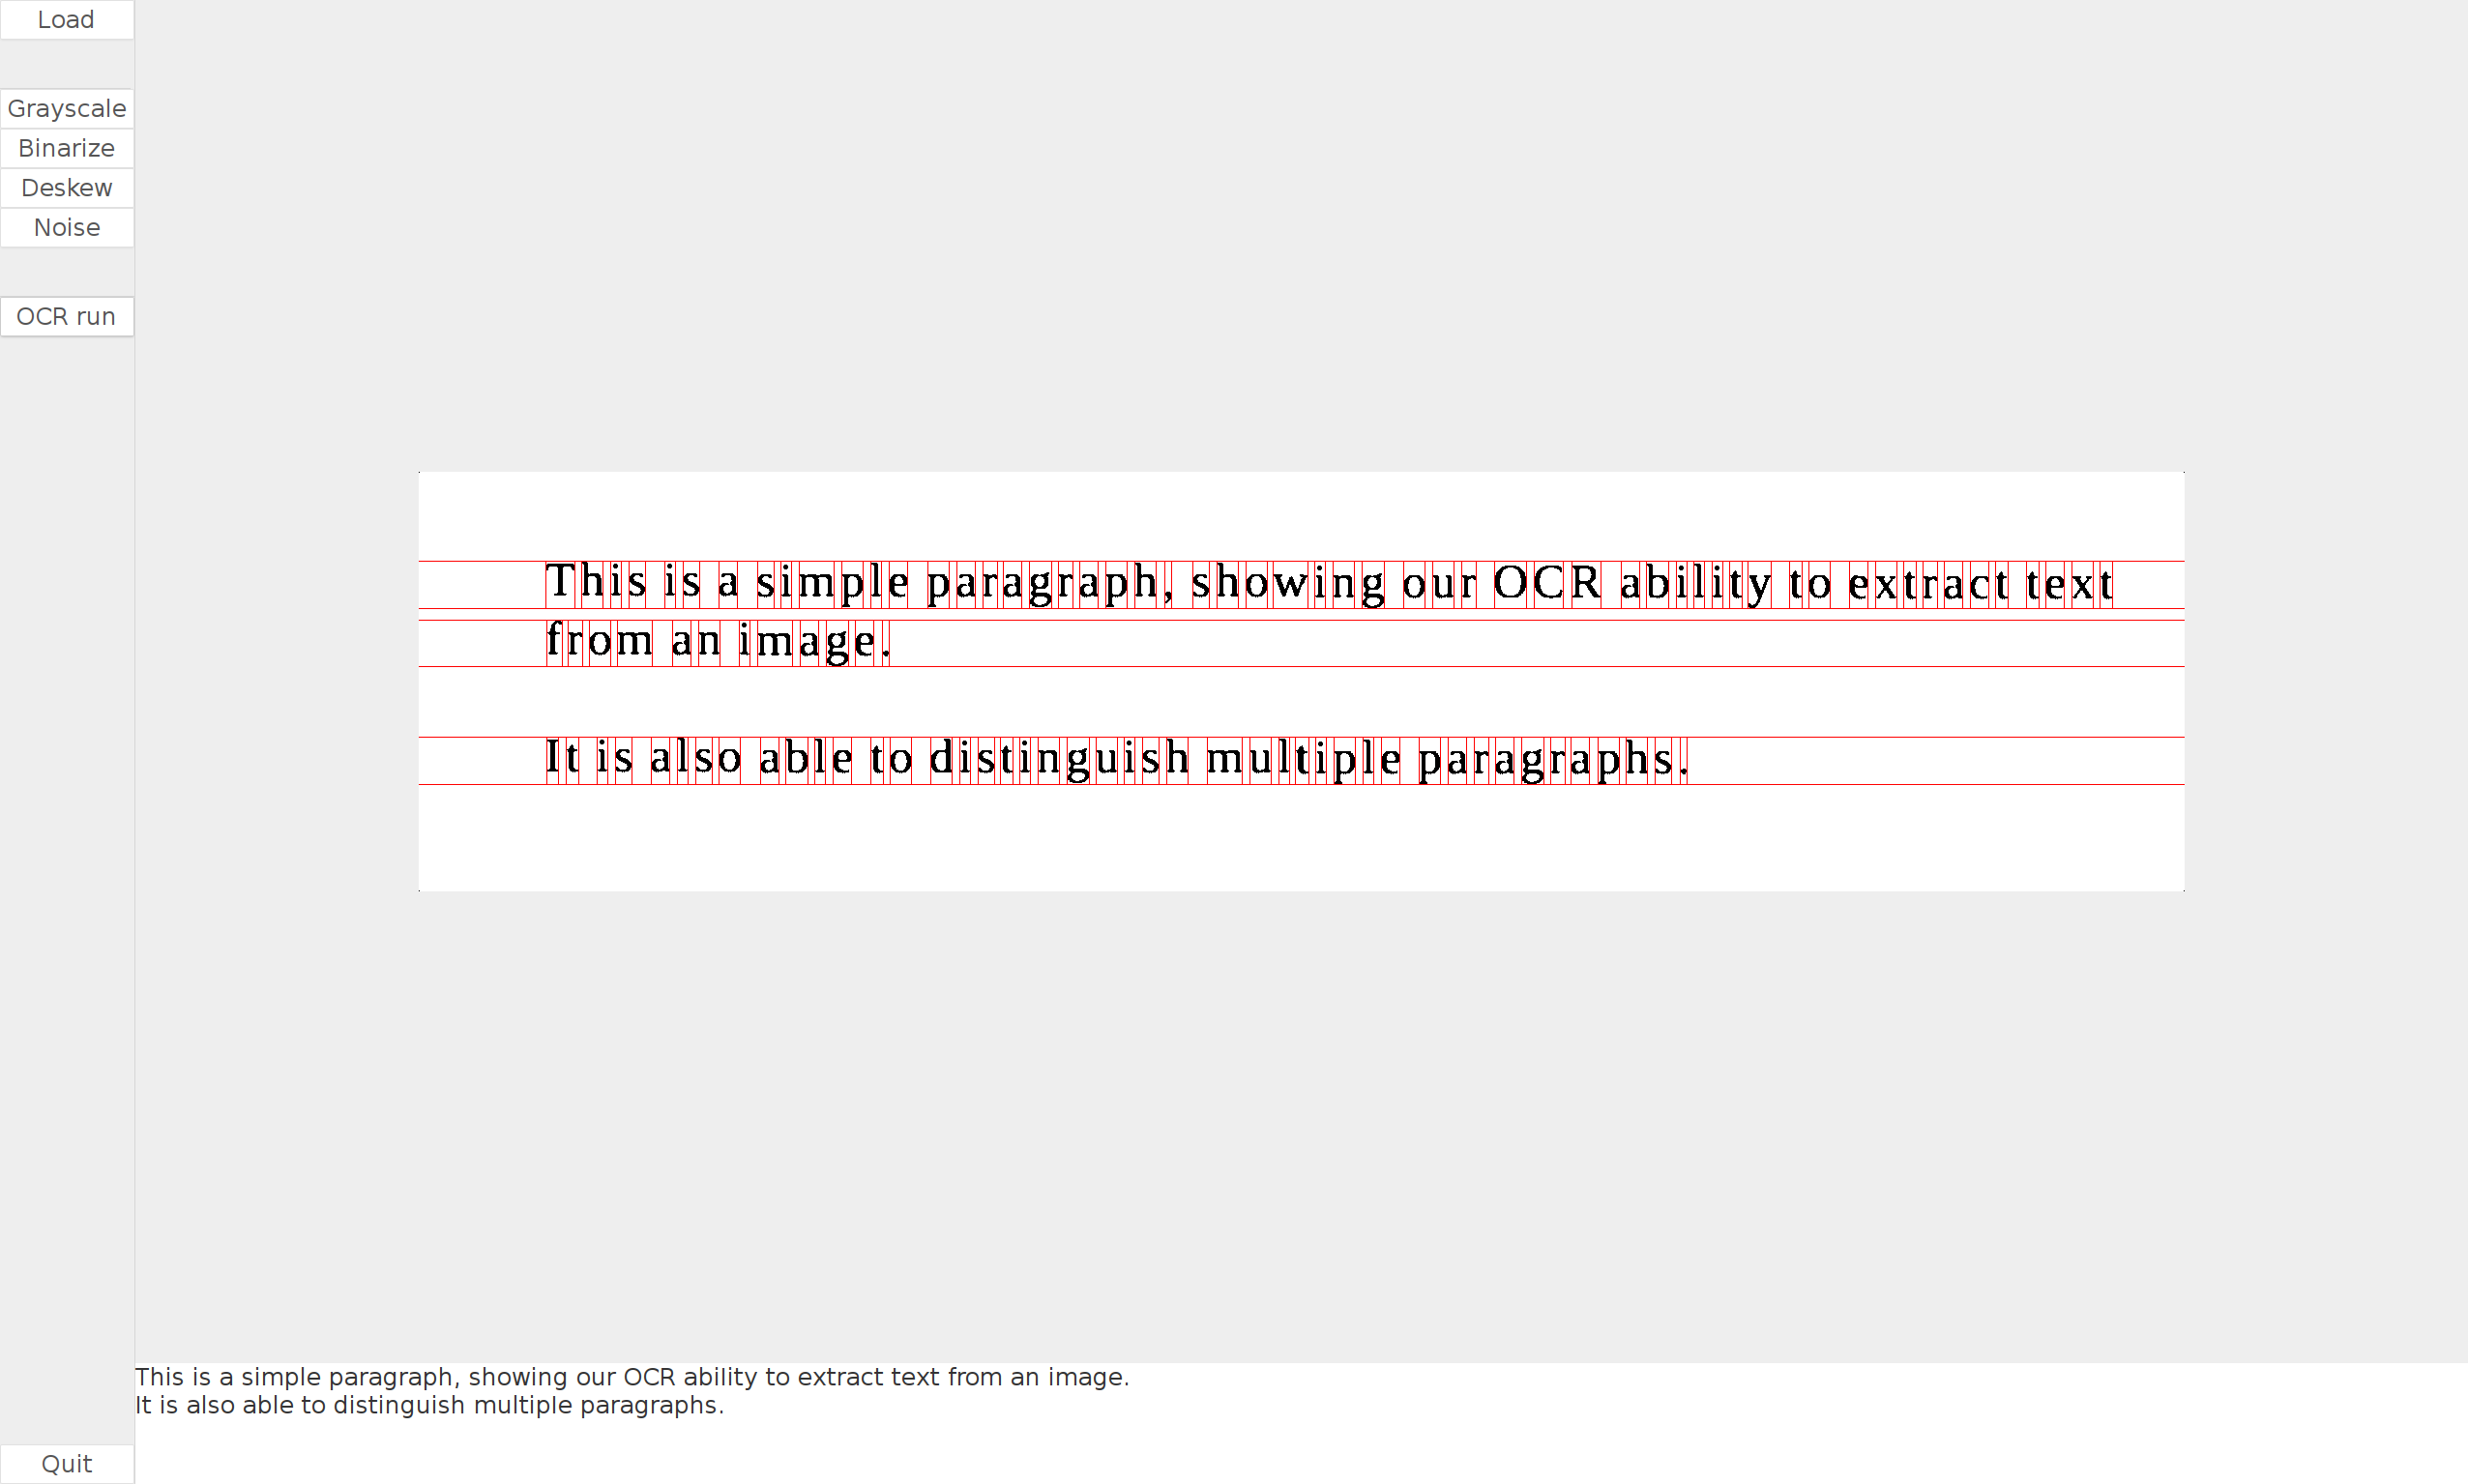
\includegraphics[width=1\textwidth]{interface2}
    \caption{Interface utilisateur}
\end{figure}
